\documentclass{article}[18pt]
\usepackage{../../../../format}
\lhead{Theory of Computation - Algorithms and Complexity}


\begin{document}
\begin{center}
\underline{\huge Revision on Algorithms and their running time}
\end{center}
\section{Algorithms}
\textbf{Algorithm}: Computational procedure that takes some value(s) as input, and produces some value(s) as output\\
\textbf{Problem}: Specifies desired relationship between input and output\\
\\
An algorithm is \textbf{correct} if for every input instance it halts with the correct output\\
A correct algorithm \textbf{solves} the problem. In this course we only consider correct algorithms
\section{Asymptotic Notation}
For two given functions $f(n)$ and $g(n)\geqslant 0$
\begin{itemize}
	\item $f(n)=\Omega(g(n))$ if $\exists c_1 > 0, n_0$ s.t
	\[
	c_{1} g(n) \leq f(n) \quad \forall n \geq n_{0}
	\]
	\item $f(n) = \mathcal{O}(g(n))$ if $\exists c_2 >0, n_0$ s.t.
	\[
	f(n) \leq c_{2} g(n) \quad \forall n \geq n_{0}
	\]
	\item $f(n) = \Theta(g(n))$ if $\exists c_1,c_2 >0, n_0$ s.t.
	\[
	c_{1} g(n) \leq f(n) \leq c_{2} g(n) \quad \forall n \geq n_{0}
	\]
	\item $f(n) = \omega(g(n))$ if $\forall c_1 > 0, \exists n_0$ s.t.
	\[
	c_{1} g(n) \leq f(n) \quad \forall n \geq n_{0}
	\]
	\item $f(n)=o(g(n))$ if $\forall c_2 >0, \exists n_0$ s.t.
	\[
	f(n) \leq c_{2} g(n) \quad \forall n \geq n_{0}
	\]
\end{itemize}
\subsection{Relationships}
For any $f(n), g(n)$
\begin{enumerate}
	\item $f(n)=\Theta(g(n))$ iff $g(n)=\Theta(f(n))$
	\item $f(n) = \Theta(g(n))$ iff $f(n)=\mathcal{O}(g(n))$ and $f(n)=\Omega(g(n))$
	\item $f(n)=\mathcal{O}(g(n))$ iff $g(n)=\Omega(f(n))$
	\item $f(n)=o(g(n))$ iff $g(n)=\omega(f(n))$
	\item $f(n)=\mathcal{O}(g(n))$ iff either $f(n)=\Theta(g(n))$ or $f(n)=o(g(n))$
	\item $f(n)=\Omega(g(n))$ iff either $f(n)=\Theta(g(n))$ or $f(n)=\omega(g(n))$
\end{enumerate}
\section{Running time}
The running time $T(I)$ of an algorithm $\alpha$ on input $I$ is the time taken by $\alpha$ on $I$ until $\alpha$ halts. We classify input according to their size.\\
\\
Size is ideally the number of bits to represent input to a real computer program, but then encoding can be done in different ways, for example encoding a graph. Thus we let the notion of size depend on the context
\subsection{Worst-case running time}
We define the worst case running time $T(n)$ of algorithm $\alpha$ on input of size n as
\[
T(n):=\max \{T(I): I \text { has size } n\}
\]
By convention, if there are no inputs of size n, we define $T(n) := 0$\\
\\
So for any input $I$ of size $n$
$$T(I)\leqslant T(n)$$
Why we are interested in worst-case running time:
\begin{itemize}
	\item It is an upper bound of the running time for any input of a given size
	\item For some algorithms, the worst case occurs fairly often
	\item The average case is often roughly as bad as the worst case
\end{itemize}
\subsection{Calculating the running time}
Let $I$ be input for algorithm $\alpha$. How to we compute $T(I)$?\\
Let the pseudocode of algorithm $\alpha$ consist of $p$ lines.\\
Assume that the execution of line i requires time 1\\
Let $q_i$ be the number of times line $i$ is executed on input $I$\\
The running time of $\alpha$ on input $I$ is
\[
T(I):=\sum_{i=1}^{p} q_{i}
\]
\subsection{Example: Insertion sort}
Let A be an array of $n$ elements. For $j= 2,3,..., n$, we let $t_j$ be the number of times the while loop test in line 4 is executes for that value of j
\begin{center}
	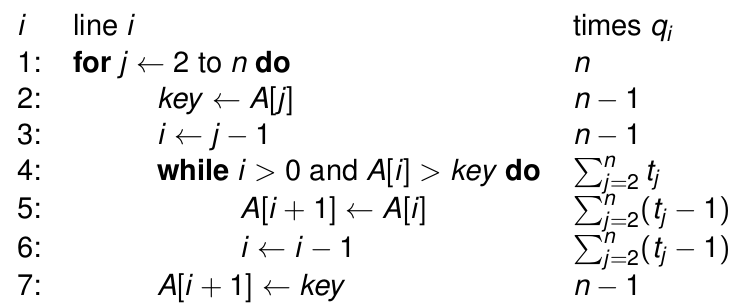
\includegraphics[scale=0.7]{Insertion-Sort}
\end{center}
Then
$$T(A)=\sum_{i=1}^{7} q_{i}=2 n-1+3 \sum_{j=2}^{n} t_{j}$$
\subsection{Worst case}
The worst case maximises $\sum_{j=2}^{n}t_j$\\
We have $t_j\leqslant j$ for all j; can we reach this bound?\\
\\
Worst case: S is in decreasing order and has distinct elements\\
\\
Then for all $2\leqslant j \leqslant n$ we have $A[i] > A[j]$ for all $1\leqslant i \leqslant j-1$\\
\\
This means that $t_j=j$ for all $2\leqslant j \leqslant n$. Hence
\[
T(n)=\frac{3}{2} n^{2}+\frac{7}{2} n-4=\Theta\left(n^{2}\right)
\]
\section{Discussion}
Reasons to use the asymptotic notation:
\begin{enumerate}
	\item Usually difficult to give precise expressions for running times. The asymptotic notation gives (tight) upper bounds in terms of natural functions
	\item From a practical point of view, we remove the dependency to specific implementation
	\item We are especially interested in the performance of algorithms for very large inputs
\end{enumerate}


\end{document}